\documentclass[12pt,english,a4paper]{article}

\usepackage[utf8]{inputenc}          % Allows UTF-8 encoded characters in the .tex-file.
\usepackage{babel,csquotes,textcomp} % Set LaTeX to structure the content following international academic standards.

% Include the TikZ-package for drawing figures.
%\usepackage{tikz}
%\usetikzlibrary{shapes.geometric,arrows}
%\usepackage{courier}

% Creates clickable hyperlinks in the PDF-document.
\usepackage{hyperref}
\usepackage{graphicx}
\usepackage{pdfpages}
\usepackage{listings}
\usepackage{wrapfig}
\usepackage{color}
\usepackage{lettrine}

\usepackage[
    backend=biber,
    style=alphabetic,
    sorting=ynt
]{biblatex}
\addbibresource{refs.bib}

\definecolor{mygreen}{rgb}{0,0.6,0}
\definecolor{mygray}{rgb}{0.5,0.5,0.5}
\definecolor{mymauve}{rgb}{0.58,0,0.82}

\lstset{ %
  basicstyle=\ttfamily\small,     
  backgroundcolor=\color{white},   % choose the background color
  breaklines=true,                 % automatic line breaking only at whitespace
  captionpos=b,                    % sets the caption-position to bottom
  commentstyle=\color{mygreen},    % comment style
  escapeinside={\%*}{*)},          % if you want to add LaTeX within your code
  keywordstyle=\color{blue},       % keyword style
  stringstyle=\color{mymauve},     % string literal style
}

\title{GPS Spoofing and the importance of time}
\author{Aril Johannes Schultzen}

\begin{document}
\maketitle
\thispagestyle{empty}
\setcounter{page}{0}
\newpage
\tableofcontents
\thispagestyle{empty}
\setcounter{page}{0}
\newpage
\thispagestyle{empty}
\setcounter{page}{0}

\begin{abstract}
Currently, this is not much more but comments and notes in order for me to write an essay, an essay meant for me to prepare for my work with my master thesis. This document does not represent the quality of the finished product in any way. Example cite \cite{KandR}
\end{abstract}

\newpage
\clearpage
\setcounter{page}{1}

\section{Global Positioning System: A short introduction}
The Global Positioning System (GPS) is a utility owned by the United States that provides its user with positioning, navigation and timing services. At the end of 60's, the U.S Navy was developing the Polaris missile, a missile capable of being launched from a submarine. One of the requirements for launching the Polaris missile was exact knowledge of the submarines position. The problem led the Navy and The Applied Physics Laboratory at Hopkins to develop the Transit system, the earliest predecessor to the GPS system \cite{SteJ}. 

Today, roughly 40 years later we are surrounded with GPS technology. In fields like emergency response, search and rescue, fleet management and even agriculture, it has become a vital tool of utmost importance to everyday operation. Satellite navigation can be found in most new cars and few phones are today sold without an internal GPS receivers. The European Space Agency estimated that there were 2 billion GPS enabled devices by 2012 \cite{ESA}. What started out as a navigation tool for the U.S navy is now used by millions, if not billions of users both civilian and military all over the globe.

\begin{figure}[hb]
  \centering
  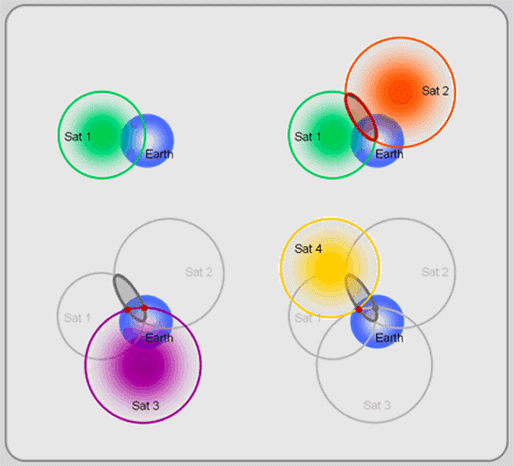
\includegraphics[scale=0.4]{trilaterate.jpg}
  \caption[GPS trilaterate figure]
   {Figure showing how GPS satellites are used to trilaterate to determine a GPS receivers position \cite{GISTRILATERATE}.}
\end{figure}

A common misconception (that is often reinforced by Hollywood action movies) is that the GPS satellites track \textit{you} by communicating with your GPS receiver. It actually works the other way around. You are, with your GPS receiver, tracking a set of satellites in order to establish your own position. At any given time, there are at least 24 GPS satellites each in its own orbit at about 11,000 nautical miles above your head \cite{GPSGOVSS}. In order for a GPS receiver to determine its position and obtain correct time, it will need 4 GPS satellites within line of sight \footnote{The line of sight requirement might seem unreasonable, but by the time the signal has reached earth, is has degraded to a minimum of -160 dBW \cite{NATINT}}.
The method used by your GPS receiver to determine its position is called \textit{trilateration}. 
Trilateration is used in geometry as a process of determining the location (absolute or relative) of point by measuring distance. It is often confused with triangulation which instead of distance, uses angles. Measuring the distance from the GPS satellites to a given position on earth is quite simple when using the equation: 
\begin{equation} Distance = Rate \times Time \end{equation} 
The equation is simple to solve, first we need the rate. In this context, the \textit{rate} is how fast the signals travel. This is equal to the speed of light (299,792,458 m/s). The time the signal has used traveling from the satellite to earth can be obtained by analyzing the signal itself. The signal contains a time stamp of when the signal was sent. By comparing this time stamp with the current time, one can calculate the age of the signal and therefore how long it has spent traveling. \cite{GPSGOVTE} 

\section{Phasor Measurement Units}
During the introduction of this article the properties of GPS as a tool for navigation was made apparent. This is however not the only use of GPS. On board of each GPS satellite there is an atomic clock. These clocks are synchronized with each other and also with clocks on the earth. Even though the use of GPS as a way to obtain correct time was not among the original design goals, it has proven useful for time critical applications. 

An example of such an application is a phasor measurement unit (PMU).A PMU analyzes the waves on the electrical grid and uses a common time source for synchronization. This synchronization allows for real-time measurements between multiple points in the grid by multiple PMU's. The common time source (and why PMU's are relevant) is obtained by using GPS.
\cite{YLJRNR}

\section{Signal interference}
\subsection{Locking on}
\subsection{Jamming}
\subsection{Spoofing}

By emitting a high-power signal at the GPS frequency, one can interfere with the signals emitted by the GPS satellites, effectively denying GPS receivers use of these signals. These signals are already weak considering their travel from space. Such an "attack", although effective, is pretty naive and easily recognized by the jammed party. After all, if you don't have a signal, you are probably being jammed. A more sophisticated approach is to emit a counterfeit signal in order to manipulate the receivers reported time or even position. IRAN, DRONE SPOOF STORY!. 


\subsection{Detection}
\subsection{Prevention}
\subsubsection{Encryption}

\newpage
\printbibliography[title={Complete Bibliography},heading=bibintoc]

\end{document}                    